% $Header$

\documentclass{beamer}

% This file is a solution template for:

% - Giving a talk on some subject.
% - The talk is between 15min and 45min long.
% - Style is ornate.

% Copyright 2004 by Till Tantau <tantau@users.sourceforge.net>.
%
% In principle, this file can be redistributed and/or modified under
% the terms of the GNU Public License, version 2.
%
% However, this file is supposed to be a template to be modified
% for your own needs. For this reason, if you use this file as a
% template and not specifically distribute it as part of a another
% package/program, I grant the extra permission to freely copy and
% modify this file as you see fit and even to delete this copyright
% notice.


\mode<presentation>
{
  \usetheme{Warsaw}
  \usecolortheme{seahorse}
  % or ...

  \setbeamercovered{transparent}
  % or whatever (possibly just delete it)
}


\usepackage[english]{babel}
% or whatever

\usepackage[latin1]{inputenc}
% or whatever

\usepackage{times}
\usepackage[T1]{fontenc}
% Or whatever. Note that the encoding and the font should match. If T1
% does not look nice, try deleting the line with the fontenc.

\usepackage{graphicx}

\title{Memristors}
\author{Charles Pittman}
\institute{The Citadel\\ELEC-424}
\date{\today}

% If you have a file called "university-logo-filename.xxx", where xxx
% is a graphic format that can be processed by latex or pdflatex,
% resp., then you can add a logo as follows:

\pgfdeclareimage[height=0.5cm]{university-logo}{university-logo.jpg}
\logo{\pgfuseimage{university-logo}}

% Delete this, if you do not want the table of contents to pop up at
% the beginning of each subsection:
% \AtBeginSubsection[]
% {
% \begin{frame}<beamer>{Outline}
%   \tableofcontents[currentsection,currentsubsection]
% \end{frame}
% }

%   If you wish to uncover everything in a step-wise fashion, uncomment
%   the following command:
%   \beamerdefaultoverlayspecification{<+->}

\begin{document}

\begin{frame}
  \titlepage
\end{frame}

\begin{frame}{Outline}
  \tableofcontents
  % You might wish to add the option [pausesections]
\end{frame}


% Since this a solution template for a generic talk, very little can
% be said about how it should be structured. However, the talk length
% of between 15min and 45min and the theme suggest that you stick to
% the following rules:

% - Exactly two or three sections (other than the summary).
% - At *most* three subsections per section.
% - Talk about 30s to 2min per frame. So there should be between about
% 15 and 30 frames, all told.

\section{Introduction}

\subsection{What is it?}

% \begin{frame}{Make Titles Informative. Use Uppercase Letters.}{Subtitles are optional.}
%   %   - A title should summarize the slide in an understandable fashion
%   %   for anyone who does not follow everything on the slide itself.

%   \begin{itemize}
%   \item
%     Use \texttt{itemize} a lot.
%   \item
%     Use very short sentences or short phrases.
%   \end{itemize}
% \end{frame}

% \begin{frame}{Make Titles Informative.}

%   You can create overlays\dots
%   \begin{itemize}
%   \item using the \texttt{pause} command:
%     \begin{itemize}
%     \item
%       First item.
%       \pause
%     \item
%       Second item.
%     \end{itemize}
%   \item
%     using overlay specifications:
%     \begin{itemize}
%     \item<3->
%       First item.
%     \item<4->
%       Second item.
%     \end{itemize}
%   \item
%     using the general \texttt{uncover} command:
%     \begin{itemize}
%       \uncover<5->{\item
%       First item.}
%       \uncover<6->{\item
%       Second item.}
%     \end{itemize}
%   \end{itemize}
% \end{frame}

\begin{frame}{What is it?}
  \center
  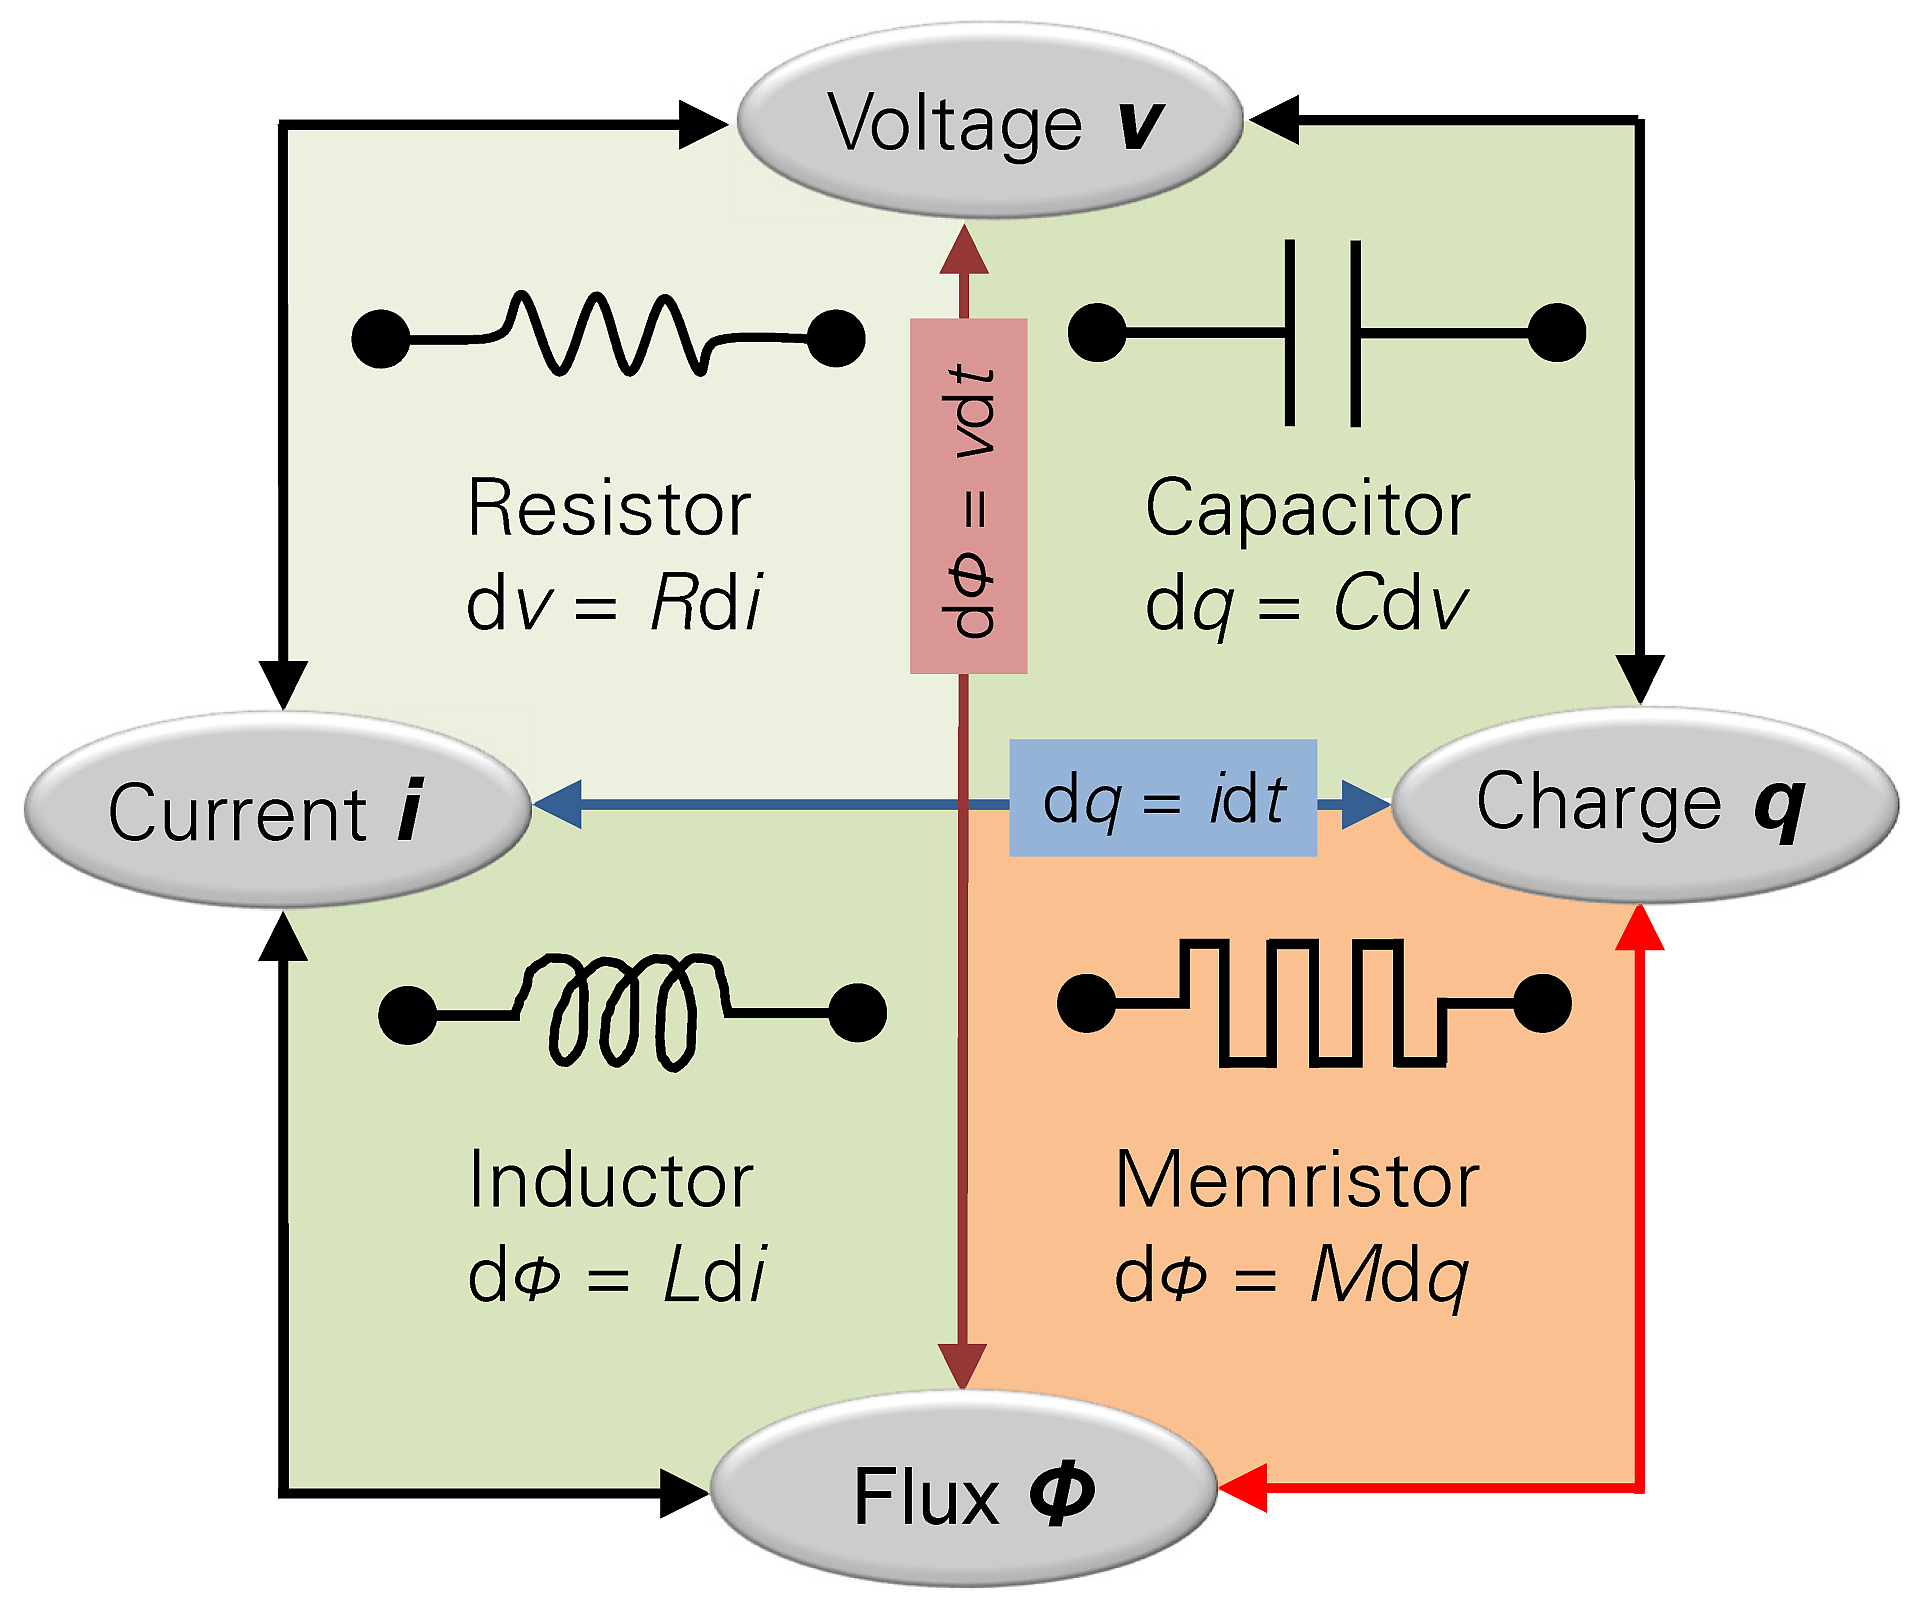
\includegraphics[height=7cm]{Memristor.png}
\end{frame}

\subsection{How does it work?}

\begin{frame}{How does it work?}
  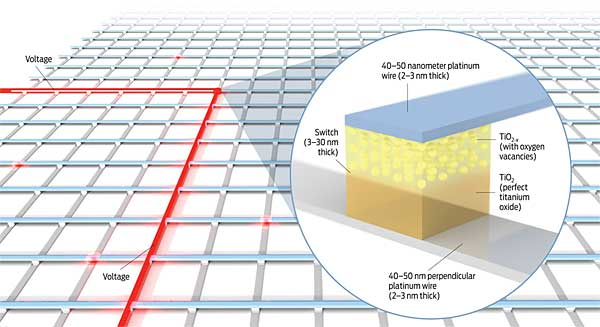
\includegraphics[height=6cm]{memristor01.jpg}
\end{frame}

\section{Applications}

\subsection{Non-Volatile Memory}

\begin{frame}{Non-Volatile Memory}
  \begin{itemize}
  \item HP's first goal
    \begin{itemize}
    \item Cross-point memory researched since the 1960s
    \end{itemize}
  \item Floating-Gate MOSFETs already used for flash memory
  \end{itemize}
\end{frame}

\subsection{Learning Circuits}

\begin{frame}{Learning Circuits}
  \begin{itemize}
  \item FGMOS also used in artificial neural networks
  \item A simple memristive circuit can react to periodic input
  \item A memristive processor is massively-parrallizable
  \end{itemize}
\end{frame}


% \subsection{Logic}

% \begin{frame}{Logic}
%     \begin{itemize}
%   \item arst
%   \end{itemize}
%   \begin{table}[h]
%     \centering
%     \caption{IMPLY}
%     \begin{tabular}{cc|c}
%       P & Q & P $\Rightarrow$ Q \\
%       \hline
%       1 & 1 & 1 \\
%       1 & 0 & 0 \\
%       0 & 1 & 1 \\
%       0 & 0 & 1
%     \end{tabular}
%   \end{table}
% \end{frame}


\section{Questions}

 \begin{frame}{}
   Questions?

%   % Keep the summary *very short*.
%   \begin{itemize}
%   \item The \alert{first main message} of your talk in one or two lines.
%   \item The \alert{second main message} of your talk in one or two lines.
%   \item Perhaps a \alert{third message}, but not more than that.
%   \end{itemize}

%   % % The following outlook is optional.
%   % \vskip0pt plus.5fill
%   % \begin{itemize}
%   % \item Outlook
%   %   \begin{itemize}
%   %   \item Something you haven't solved.
%   %   \item Something else you haven't solved.
%   %   \end{itemize}
%   % \end{itemize}
 \end{frame}

\end{document}
